\documentclass{article}
\usepackage[legalpaper, portrait, margin=1in]{geometry}
\usepackage{graphicx} % Required for inserting images
\usepackage{hyperref}
\usepackage{amsmath}
\usepackage{listings}
\usepackage{xcolor}
\usepackage{algorithm} % For pseudocode
\usepackage{algpseudocode} % For pseudocode
\usepackage[font=small,labelfont=bf]{caption}
\usepackage{pgfplots}
\usepackage{float}
\usepackage[top=0.75in, bottom=0.75in, left=0.5in, right=0.5in]{geometry}
\usepackage{pgfplots}

\lstset{
    basicstyle=\ttfamily\small,
    keywordstyle=\color{blue},
    commentstyle=\color{green!50!black},
    stringstyle=\color{red},
    breaklines=true,
    showstringspaces=false,
    frame=single,
}
\hypersetup{
    colorlinks=true,
    urlcolor=blue,
    linkcolor=blue,
    citecolor=red
}
\usepackage{algorithm} % For pseudocode
\usepackage{algpseudocode} % For pseudocode
\setlength{\parindent}{0pt}
\setlength{\parskip}{1em}

\title{Pickleball Flight Final Report}
\author{Maxwell Feng (mzf), Daniel Zhang (dzhang3)\\Website: \href{https://dzhang95.github.io/pickleball/}{https://dzhang95.github.io/pickleball/}}
\date{December 8th 2025}

\begin{document}

\maketitle

\pagebreak

\section{Summary}

We developed a particle-based collision simulation in C++ to model the motion of a ball interacting with surrounding air particles. Our system includes both sequential and parallel implementations, as well as a real-time visualization using OpenGL. We evaluate the computational performance of our simulator on the GHC machines and demonstrate meaningful speedups from parallelization while preserving accurate collision behavior.

\section{Background}

\subsection{Problem Description}

We would like to consider the computationally-intensive problem of particle collision and analyze what speedups we can achieve using CUDA. Specifically, we would like to simulate a ball flying through the air and how air resistance, which we will abstract as collisions with air particles, affects the trajectory/velocity of the ball. Software like Ansys CFD (Computational Fluid Dynamics) can simulate golf balls or other objects flying through the air with air particle collisions. However, these software are typically not open-sourced, and we would like to achieve high speedups for these similar problems.



\subsection{Assumptions}

Before diving deeper into the problem, we list some key assumptions we are making:
\begin{itemize}
\item Each air particle is a circle. There are an unimaginable and incomputable number of air particles in a closed space, so we will abstract a group of air particles as a circular air parcel.
\item The pickleball is a simple circle without any holes.
\item There can be small vacuums (areas without any air particles) in the world.
\item We cannot change the size of the world, AKA a pickleball court and the surrounding area.
\item We can change the "problem size" via particle count.
\item We will calculate the world as 2D. The visualization displays an x and y axis, which shows the pickleball court (top-down view).
\item Air particles can escape our world.
\end{itemize}

\subsection{Formalizing Collisions}

The main computational cost in this project involves collisions. We now describe the mathematics behind how we detect and calculate collisions.

We consider two air particles with positions and velocities
\[
\mathbf{x}_1 = (x_1, y_1), \qquad \mathbf{x}_2 = (x_2, y_2), \qquad
\mathbf{v}_1 = (v_{1x}, v_{1y}), \qquad \mathbf{v}_2 = (v_{2x}, v_{2y}),
\]
and masses \(m_1, m_2\). Each particle has radius \(r = \texttt{airParticleRadius}\).

First, we compute the distance between the particles:
\[
\Delta x = x_2 - x_1, \qquad
\Delta y = y_2 - y_1, \qquad
d = \sqrt{(\Delta x)^2 + (\Delta y)^2}.
\]
Between either two air particles or air particle and ball, we define the minimum non-overlapping distance
\[
d_{air} = 2r, \qquad d_{ball} = r + R
\]
If
\[
0 < d < d_{air}, \qquad 0 < d < d_{ball}
\]
then the particles overlap. We define the collision normal
\[
\hat{\mathbf{n}} = (n_x, n_y) = \frac{1}{d}(\Delta x, \Delta y).
\]
The overlap amount is
\[
\delta = d_{air} - d, \delta = d_{ball} - d,
\]
so each particle is moved by half the overlap along \(\hat{\mathbf{n}}\):
\[
\mathbf{x}_1' = \mathbf{x}_1 - \frac{\delta}{2}\,\hat{\mathbf{n}}, \qquad
\mathbf{x}_2' = \mathbf{x}_2 + \frac{\delta}{2}\,\hat{\mathbf{n}}.
\]

Next, we compute the relative velocity and its component along the normal:
\[
\mathbf{v}_{\text{rel}} = \mathbf{v}_2 - \mathbf{v}_1, \qquad
v_{\text{rel},n} = \mathbf{v}_{\text{rel}} \cdot \hat{\mathbf{n}}.
\]
We only apply an impulse if the particles are moving towards each other, i.e.,
\[
v_{\text{rel},n} < 0.
\]

Let \(e\) be the coefficient of restitution (in the code, \(e = 0\) for a perfectly inelastic collision). The scalar normal impulse magnitude is
\[
J_n = -\,\frac{(1 + e)\,v_{\text{rel},n}}{\frac{1}{m_1} + \frac{1}{m_2}}.
\]
The impulse vector is
\[
\mathbf{J} = J_n\,\hat{\mathbf{n}}.
\]
Finally, the post-collision velocities are updated by
\[
\mathbf{v}_1' = \mathbf{v}_1 + \frac{\mathbf{J}}{m_1}, \qquad
\mathbf{v}_2' = \mathbf{v}_2 - \frac{\mathbf{J}}{m_2}.
\]

Note that since $m$ for air particles is extremely small, we have that $\frac{\mathbf{J}}{m}$ can blow up extremely large. Thus, we let
\[
k = \texttt{AIR\_AIR\_IMPULSE\_SCALE\_FACTOR}
\]
be a tuning scale factor and get 
\[
\mathbf{v}_1' = \mathbf{v}_1 + k\frac{\mathbf{J}}{m_1}, \qquad
\mathbf{v}_2' = \mathbf{v}_2 - k\frac{\mathbf{J}}{m_2}.
\]

This tuning scale factor sacrifices correctness, but it helps rendering and visualizing the air particles.

Once we have calculated the velocity for each particle, we can compute its position in the next frame (after the next timestep) simply by

\[
x_{new} = x_{old} + v_x \cdot t, \qquad y_{new} = y_{old} + v_y \cdot t
\]

\subsection{Formalizing Spin}

To model spin, we treat the ball as a rigid body with both translational and rotational degrees of freedom. At each contact with an air particle, we compute the surface velocity of the ball at the contact point as the sum of the translational velocity and the rotational contribution $\mathbf{v}_{\text{rot}} = \omega \times \mathbf{r}_c$, where $\omega$ is the ball's angular velocity and $\mathbf{r}_c$ is the vector from the center of the ball to the contact point. The relative velocity between the particle and this surface point is then decomposed into normal and tangential components. A normal impulse $J_n$ prevents interpenetration, while a frictional tangential impulse $J_t$ (clamped by a Coulomb friction bound $|J_t| \le \mu |J_n|$) both changes the particle's velocity and applies a torque $\tau = \mathbf{r}_c \times \mathbf{J}$ to the ball, updating its spin. In addition to these discrete collision impulses, we include a continuous Magnus-effect term with acceleration proportional to $\omega \times \mathbf{v}$ to capture the macroscopic curvature of the ball's trajectory through the air.


\subsection{Data Structures}

For each air particle, we would like to track both its location and velocity. Additionally, we would like information about its mass for impulse calculations. Thus, we can construct a single array of \texttt{AirParticle} structs, which includes all the generated air particles. For each particle, we can individually compute its change in velocity based on collisions with other particles and the ball, as described in section 2.3. Further details on operations performed on particles is discussed in section 3.3 (Sequential Simulation). The ball can be represented the same as the air particle but with a larger mass and radius.

For rendering, the primitive for OpenGL is triangles, so we use several rotated triangles to approximate a circle. Air particle positions are stored in GPU-resident buffers (VBOs), which are updated each frame either directly from device memory via CUDA or through CPU for serial implementation. Once updated, these buffers are consumed by OpenGL instanced draw calls to render all particles in parallel. In the CUDA-rendering mode, we additionally support rasterizing particles into an offscreen RGBA image entirely on the GPU, which is then copied back and blended over the scene. This design minimizes CPU–GPU data transfer and leverages GPU parallelism to maintain smooth real-time visualization.

Our algorithm takes in a list of particles (and ball) with positions, velocities, and masses, and outputs an updated list of particles with new positions and velocities.

\subsection{Workload and Computational Costs}

The dominant source of computation in our simulator is collision detection, collision resolution, and rendering the objects. Initially, in each frame, every air particle must be checked for intersection with every other particle. Because we did not use any spatial partitioning or broad-phase culling initially, this results in a naive all-pairs comparison. With $N$ air particles, the number of collision checks scales as

\[
\mathcal{O}(N^2) = \frac{N(N-1)}{2},
\]

which quickly becomes expensive as $N$ increases.

Additionally, each detected collision incurs further cost due to (1) computing the collision normal and penetration depth and (2) applying an impulse update to both particles. These operations include multiple vector calculations, normalization, and conditional checks for physically valid interactions.

The ball--air interactions add another $\mathcal{O}(N)$ workload per frame, where each air particle is tested against the ball for potential contact.

Together, this summarizes the total workload for the "physics" step of the per-frame workload. This is summarized as follows.

\[
Tp(N) = \mathcal{O}(N^2) + \mathcal{O}(N) \approx \mathcal{O}(N^2).
\]

There is still additional work for the frame however, namely the actual rendering of all our particles. This step contains the device raster kernel, which works out to $\mathcal{O}(N)$, and the copy of the frame buffer from the device to the host, which works out to $\mathcal{O}(ImageArea)$. So the total work for the rendering portion is as follows.

\[
Tr(N) = \mathcal{O}(N) + \mathcal{O}(ImageArea)
\]

As a result, given that N is much more significant than the image size, the total work for one frame is

\[
T(N) = Tp(N) + Tr(N) = \mathcal{O}(N^2) + \mathcal{O}(N) + \mathcal{O}(N) + \mathcal{O}(ImageArea) \approx \mathcal{O}(N^2).
\]

Within a single frame, the simulation exhibits significant data parallelism. Each air particle update is independent, and each air--air collision affects only the two particles involved. The only global dependency arises in the ball--air collision phase, where impulses applied by individual particles must be accumulated into a shared ball velocity and angular momentum update. This can be safely parallelized using per-thread reductions. While the simulation remains sequential across frames, the dominant workload inside each frame can be parallelized effectively.

Our workload is highly data-parallel, making it well suited for GPU execution. CUDA allows us to launch thousands of lightweight threads, enabling each particle—or particle pair—to be processed independently. While SIMD execution could be used for this project, CUDA provides significantly higher floating-point throughput and memory bandwidth, which are critical for the many vector operations and memory accesses in collision resolution.

\subsection{Spatial Partitioning}

After we confirmed that the code was working, we then proceeded to implement spatial partitioning of the world so that we don't have $\mathcal{O}(N^2)$ complexity when checking for collisions. With spatial partitioning, the world is split into multiple cells. Instead of checking every particle with every other particle, we only check particles that are in the same cell or in a neighboring cell. This greatly reduced the complexity of the collision checking step to approximately $\mathcal{O}(N)$.

Since the ball-air interactions did not use spatial partitioning, it still had $\mathcal{O}(N)$ complexity. Therefore, the physics per-frame workload now was

\[
T(N) = \mathcal{O}(N) + \mathcal{O}(N) \approx \mathcal{O}(N).
\]

And the total workload of one frame was now

\[
T(N) = Tp(N) + Tr(N) = \mathcal{O}(N) + \mathcal{O}(N) + \mathcal{O}(N) + \mathcal{O}(ImageArea) \approx \mathcal{O}(N).
\]


\section{Approach}

\subsection{Tech Stack}

We used C++ for the codebase and sequential simulator, CUDA for the parallel simulator, and GLFW and GLEW libraries for OpenGL rendering.

The code was benchmarked on the GHC (Gates Hillman Clusters) machines with an Intel i7-9700 CPU and an NVIDIA GeForce RTX 2080 GPU.

Videos of the simulation were screenrecorded and then edited with CapCut.

\subsection{Invocation and Variables}

Our simulation can be ran by the following command:

\begin{verbatim}
    ./renderer -t --cuda --cuda-no-fallback -p N --ball-vx X --ball-vy Y --ball-spin OMEGA
\end{verbatim}

The arguments are described below:

\begin{itemize}
    \item t: enables ball trajectory visualization
    \item cuda: enables CUDA
    \item cuda-no-fallback: aborts if CUDA not available; if not invoked, then code falls back to CPU execution
    \item p: number of air particles to spawn
    \item X: initial x velocity of the ball (in m/s)
    \item Y: initial y velocity of the ball (in m/s)
    \item OMEGA: initial angular velocity of the ball (in rad/s)
\end{itemize}

In our program, we also keep some constants to emulate a real pickleball scenario:

\begin{itemize}
    \item Mass of the ball: 0.026 kg
    \item Radius of the ball: 0.185 m
    \item Mass of air particles: 0.00000001 kg
    \item Radius of air particles: $1 \cdot 10^{-8}$ m
    \item Size of the court: 13.4 x 6.1 m
\end{itemize}

Some of these values, like radius or mass, are unrealistic for our situation, but due to floating number restraints and visualization purposes, we increase these values.

\subsection{Sequential Simulation}

In order to have a baseline of performance, we first implemented the simulation sequentially. This version of the program runs on the CPU and will be invoked if you do not supply the cuda flag.
We split the application's main rendering loop into two steps, physics and rendering. These steps are then further split down as follows:
\begin{itemize}
\item Physics
\begin{itemize}
\item Update ball position
\item Air-air 
\begin{itemize}
\item Collision detection
\item Collision resolution
\end{itemize}
\item Ball-air
\begin{itemize}
\item Collision detection
\item Collision resolution
\end{itemize}
\item Calculate the Magnus effect for spin
\end{itemize}
\item Rendering
\begin{itemize}
\item Draw the court
\item Draw air particles
\item Draw the net
\item Draw the ball
\item Draw the ball's path, if flag supplied
\end{itemize}
\end{itemize}

\subsubsection{Initial Attempt}

The algorithm for calculating new positions for each frame is described in the following pseudocode:

\begin{algorithm}[H]
\caption{Sequential Simulation}
\begin{algorithmic}[1]
\State Update the ball's position based on velocity
\For{any two particles in particle list}
\State Check if they collide by checking distance between centers
\If{collision detected}
\State Calculate impulses and change momentum to calculate new velocities of particles
\EndIf
\EndFor
\For{particles in particle list}
\State Check if the air particle intersects with the ball
\If{collision detected}
\State Calculate impulses and change momentum to calculate new velocities of ball and particle
\State Calculate effect of spin on ball and particle
\EndIf
\EndFor
\end{algorithmic}
\end{algorithm}

Note that for calculating collisions, we perform two for loops over all particles. Based on the pseudocode structure, we already have some notion of parallelizing over each particle. This sequential algorithm is very naïve and is subject to many different possible optimizations.

\subsubsection{Journey and Optimizations}

We realized that our bottleneck is the $O(N^2)$ cost from computing air-air collisions. We drew inspiration from the circle renderer from assignment 2 on how to improve our sequential computation speed. We can partition our world into cell lists and determine which cell each particle falls in. Then, our time complexity reduces since for each particle, we only need to check its neighboring cells.

Implementation-wise, we first iterate over all particles to hash each particle to its cell. We keep track of the counts for each cell and which particles (so we can extract velocity information). Also, we ensure that the cell size is slightly larger than the diameter so that collisions can only occur between neighboring particles.

\subsubsection{Final Pseudocode}

With our new optimization, we have our final sequential algorithm:

\begin{algorithm}[H]
\caption{Optimized Sequential Simulation}
\begin{algorithmic}[1]
\State Update the ball's position based on velocity
\For{any particle in particle list}
\State Hash the particle to its cell
\EndFor
\For{particles in particle list}
\State Check neighboring cells for any particles
\State If there are particles in neighboring cells, check for collisions and calculate new velocities based on impulses
\EndFor
\end{algorithmic}
\end{algorithm}

\subsubsection{Implementation Details}

Although we give a brief outline on the sequential algorithm, we would like to point to specific areas in the code to help the reader navigate the codebase. All sequential code is located in the renderer.cpp file.

In our main rendering loop, we begin our algorithm that we separated into two stages: simulation and rendering:

\begin{lstlisting}
// --- Physics section (timed) ---
simulatePhysics(timestep, airParticles, use_cuda_requested, spinDeltaAccumulator, showPath);

// Clear the screen and render (timed)
renderFrame(window, shaders, airParticles, timestep, showPath);
\end{lstlisting}

For the simulation phase, we begin by calculating the position of the ball and particles

\begin{lstlisting}
    circleX += circleVelX * timestepSize;
    circleY += circleVelY * timestepSize;
    for (size_t i = 0; i < airParticles.size(); i++) {
        airParticles[i].x += airParticles[i].velX * timestepSize;
        airParticles[i].y += airParticles[i].velY * timestepSize;
    }
\end{lstlisting}

We then perform our cell list optimization by hashing particles to their respective cell:

\begin{lstlisting}
    for (size_t i = 0; i < airParticles.size(); ++i) {
        int64_t key = cell_key(airParticles[i].x, airParticles[i].y);
        cellMap[key].push_back(i);
    }
\end{lstlisting}

We then iterate over all particles to check for collisions with neighbors:

\begin{lstlisting}
    for (size_t i = 0; i < airParticles.size(); ++i) {
        AirParticle &p1 = airParticles[i];
        // compute cell coords for p1
        int base_cx = (int)std::floor((p1.x + rectHalfWidth) / cellSize);
        int base_cy = (int)std::floor((p1.y + rectHalfHeight) / cellSize);
    
        for (int dy = -1; dy <= 1; ++dy) {
            for (int dx = -1; dx <= 1; ++dx) {
                ...
                // collision detected
                if (distance < minDistance && distance > 0.0001f) {
                    ...
                    p1.velX += impulseX * invM1;
                    p1.velY += impulseY * invM1;
                    p2.velX -= impulseX * invM2;
                    p2.velY -= impulseY * invM2;
                }
            }
        }
\end{lstlisting}

We then repeat collision detection for air particles with the ball, which essentially has the same logic as before (except we don't need the spatial grid):

\begin{lstlisting}
    for (size_t i = 0; i < airParticles.size(); i++) {
            AirParticle& particle = airParticles[i];
            float dx = particle.x - circleX;
            float dy = particle.y - circleY;
            float distance = sqrtf(dx * dx + dy * dy);
            float minDistance = BALL_RADIUS + airParticleRadius;
            if (distance < minDistance && distance > 0.0001f) {
                ...
            }
    }
\end{lstlisting}

We then calculate the Magnus effect on the ball, which concludes the simulation phase:

\begin{lstlisting}
    const float k_magnus = 0.0005f;
    float magnusAx = k_magnus * (-circleSpin * circleVelY) / BALL_MASS;
    float magnusAy = k_magnus * ( circleSpin * circleVelX) / BALL_MASS;
    circleVelX += magnusAx * timestepSize;
    circleVelY += magnusAy * timestepSize;
\end{lstlisting}

For the rendering phase, we simply abuse the OpenGL library to clear and render the screen. Here are some code snippets that draw our scene:

\begin{lstlisting}
    // clear scene
    glClearColor(0.1f, 0.1f, 0.1f, 1.0f);
    glClear(GL_COLOR_BUFFER_BIT);
    
    // draw court
    glUseProgram(shaders.rectangleShader);
    float rect_w_ndc = WORLD_W * NDC_SCALE;
    float rect_h_ndc = WORLD_H * NDC_SCALE;
    renderRectangle(0.0f, 0.0f, rect_w_ndc, rect_h_ndc);
    
    // draw particles
    glUseProgram(shaders.airParticleShader);
    int ninstances = (int)airParticles.size();
    if (ninstances > 0) {
        ...
        int loc = glGetUniformLocation(shaders.airParticleShader, "u_instance_scale");
        glUniform1f(loc, airParticleRadius * NDC_SCALE);
        glBindVertexArray(g_particleVAO);
        glDrawArraysInstanced(GL_TRIANGLES, 0, vertexCount, ninstances);
        glBindVertexArray(0);
    }

    // draw ball
    glUseProgram(shaders.circleShader);
    renderCircle((circleX - world_cx) * NDC_SCALE, (circleY - world_cy) * NDC_SCALE, BALL_RADIUS * NDC_SCALE, 32);
\end{lstlisting}

\subsection{Parallelizing Collisions}

\subsubsection{Journey and Optimizations}

To create the parallel version of our code, we first modified our physics step to be able to run on CUDA without the optimized spatial partitioning approach. We also added a flag to easily switch between the sequential implementation and the parallel implementation. Creating the initial CUDA code was relatively simple, as the logic was still the same.

After confirming that the physics step did in fact have big gains when moved to CUDA, we realized that our render step was now the big bottleneck. That step was still running on the CPU and dominated the runtime now. So obviously, the next thing we wanted to do was try and optimize the render step as much as we could. We then created a CUDA version of the render step that would run if the cuda flag was supplied. However, this did not provide much speedup if any. The computations required for this step were not that intensive, and the amount of data that needed to copied back and forth between device and host proved to be a significant memory bottleneck.

Next, we applied the same spatial grid optimization that was done to the sequential implementation. This gave us MASSIVE improvements for large particle counts, as will be shown later.

Other optimizations and changes we wanted to try but ran out of time for:
\begin{itemize}
\item Reinspect atomics to determine if they are necessary
\item Finetune grid parameters
\item Use Thrust for sorting
\item Only transfer parts of the image that changed from device to host
\item Improve memory layout on device
\end{itemize}

\subsubsection{Final Pseudocode}

The serial algorithm more or less stayed the same.

The parallel algorithm for calculating new positions for each frame is described in the following pseudocode:

\begin{algorithm}[H]
\caption{Parallel Physics Simulation (CUDA)}
\begin{algorithmic}[1]
\State Update the ball’s position based on velocity
\State Copy particle data to device
\State Build spatial grid on GPU to find nearby neighbors
\ForAll{particles \textbf{in parallel}}
    \State Check collisions with neighbors in nearby grid cells
    \If{air--air collision detected}
        \State Apply collision response to particle velocities
    \EndIf
    \State Check collision with ball
    \If{collision detected}
        \State Apply impulses and friction to update particle
        \State Atomically accumulate equal-and-opposite impulse and spin on ball
    \EndIf
    \State Handle boundary constraints for particle
\EndFor
\State Copy updated particle data and ball impulse/spin back to host
\State Apply continuous Magnus effect to ball
\end{algorithmic}
\end{algorithm}

\subsubsection{Implementation Details}

Again, we divide the algorithm into simulate and render phases. However, we compute collisions on device, keep the results on device, and render using CUDA to write directly into the VBO buffer. The main method we use is cuda\_physics\_run\_device, which can be found in cuda\_kernels.h:

\begin{lstlisting}
bool cuda_physics_run_device(float* px, float* py, float* pvx, float* pvy, int n, float* ballState, float dt);
\end{lstlisting}

This method uses two main CUDA kernels:

\begin{lstlisting}
    // build cell lists
    kernel_build_cell_lists<<<blocks, threads>>>(g_px, g_py, n, g_numCellsX, g_numCellsY, CUDA_CELL_SIZE, RECT_HALF_W_CU, RECT_HALF_H_CU, g_cell_counts, g_cell_lists, CUDA_MAX_PARTICLES_PER_CELL);

    // check neighbors
    kernel_physics_neighbors<<<blocks, threads>>>(g_px, g_py, g_pvx, g_pvy, n, ballX, ballY, ballVelX, ballVelY, ballSpin, g_numCellsX, g_numCellsY, CUDA_CELL_SIZE, RECT_HALF_W_CU, RECT_HALF_H_CU, g_cell_counts, g_cell_lists, CUDA_MAX_PARTICLES_PER_CELL, g_impulse_x, g_impulse_y, g_spin_accum, dt);
\end{lstlisting}

The first kernel maps a thread to each particle and performs the hashing of each particle. The second kernel iterates over all neighbors in the cell lists and computes collisions and resulting states. The implementation for these kernels is very similar to the sequential version described in section 3.3.4 Implementation Details.

\subsubsection{Mapping}

For building the spatial grid and checking for neighbors, we parallelize across particles. Each block has 256 threads, and each thread handles a particle.

\begin{lstlisting}
const int threads = 256;
int blocks = (n + threads - 1) / threads;
kernel_physics_neighbors<<<blocks, threads>>>(...);
\end{lstlisting}

We also maintain three global accumulators on the device:
\[
\texttt{g\_impulse\_x}, \texttt{g\_impulse\_y}, \texttt{g\_spin\_accum},
\]
which are updated with \texttt{atomicAdd} to avoid race conditions. Since all particles can potentially affect these variables (collisions with the ball), we make them global across the device.

Additionally, when computing particle and ball states, if we also render on GPU, then transferring the data back to CPU and then back to device is a waste of bandwidth. By keeping the data on device, both physics and rendering are primarily on the GPU, and PCIe transfer overhead is reduced.

\section{Results}

\subsection{Evaluation Metrics}

Our first evaluation metric is speedup when using CUDA compared to vanilla sequential execution on CPU. For smaller test sizes (around 3000 particles), moving computations to the GPU may actually hurt our runtime due to limited bandwidth and relatively low compute times. Ideally, we would like to test speedup for sequential vs. parallel on larger test sizes. However, running past 3000 particles sequential was too slow for us to reasonably run comparisons. Since the CPU implementation becomes prohibitively slow beyond this range while the GPU continues to scale, parallel speedup for this project is extremely powerful.

Also, we would like to analyze speedup with respect to number of air particles we spawn in. We would like to see how speedup scales with the number of particles. More specifically, we want to compare our implementation before adding the spatial grid and after. Since our time complexity is linear with respect to the number of particles after adding the spatial grid, we hypothesize that the computation time for collisions will scale approximately linearly as we increase the number of air particles. 

\subsection{Experimental Setup}

For experiments, we varied the number of air particles from 1,000 to 1,000,000 in multiples of 10. Additionally, since there are not as many collisions at the beginning of the simulation, we allow the program to run for several frames before collecting timing information. For performance, we measure total milliseconds for frames and average ms per frame (for both physics computations and rendering time), GPU utilization, and GPU memory usage.

We also compared the runtime before and after the spatial grid optimization.

\subsection{Graphs}
\subsubsection{Varying Problem Size}

\begin{center}

\begin{subfigure}{\textwidth}
\centering
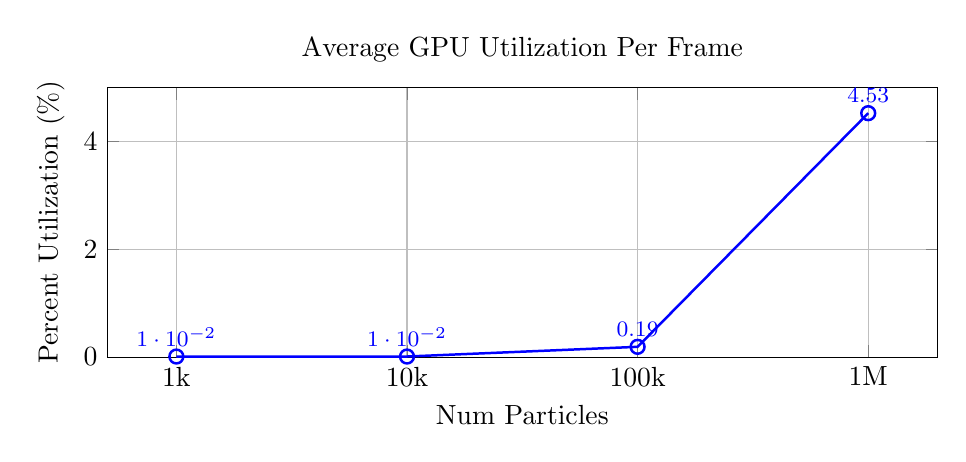
\begin{tikzpicture}
\begin{axis}[
  width=\linewidth, height=5cm,
  xlabel={Num Particles}, ylabel={Percent Utilization (\%)},
  grid=both,
  symbolic x coords={1k,10k,100k,1M},
  xtick=data,
  ymin=0, ymax=5,
  nodes near coords,
  every node near coord/.append style={font=\footnotesize,anchor=south},
  title={Average GPU Utilization Per Frame},
]
\addplot+[mark=o, line width=0.9pt, mark size=2.5pt]
  coordinates {(1k, 0.01) (10k, 0.01) (100k, 0.19) (1M, 4.53)};
\end{axis}
\end{tikzpicture}
\end{subfigure}


\hfill

\begin{subfigure}{\textwidth}
\centering
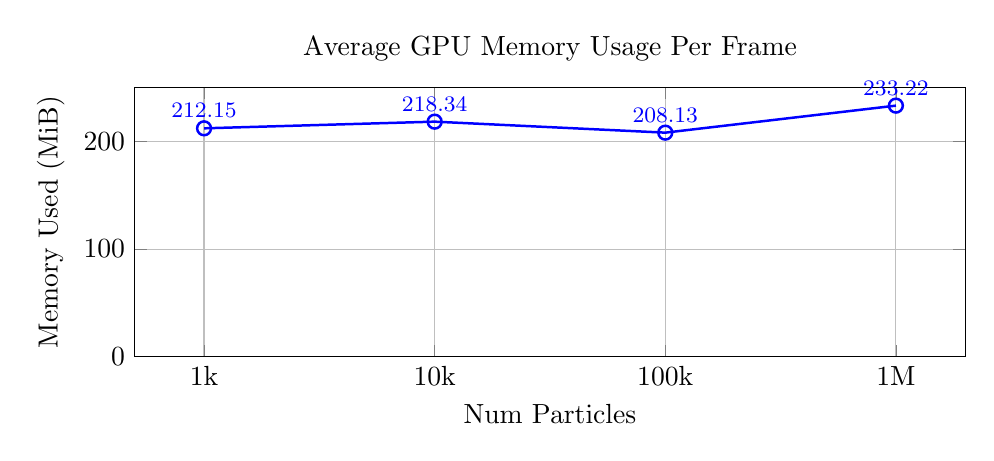
\begin{tikzpicture}
\begin{axis}[
  width=\linewidth, height=5cm,
  xlabel={Num Particles}, ylabel={Memory Used (MiB)},
  grid=both,
  symbolic x coords={1k,10k,100k,1M},
  xtick=data,
  ymin=0, ymax=250,
  nodes near coords,
  every node near coord/.append style={font=\footnotesize,anchor=south},
  title={Average GPU Memory Usage Per Frame},
]
\addplot+[mark=o, line width=0.9pt, mark size=2.5pt]
  coordinates {(1k, 212.15) (10k, 218.34) (100k, 208.13) (1M, 233.22)};
\end{axis}
\end{tikzpicture}
\end{subfigure}


\hfill

\begin{subfigure}{\textwidth}
\centering
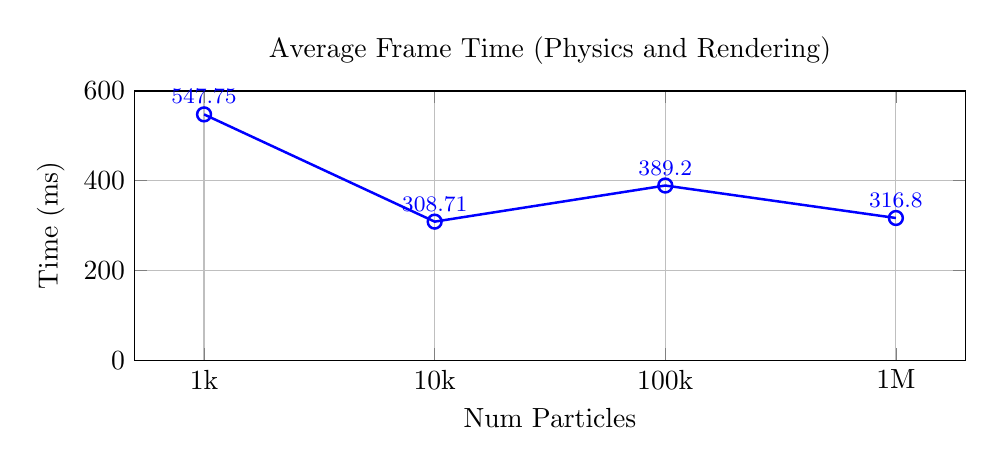
\begin{tikzpicture}
\begin{axis}[
  width=\linewidth, height=5cm,
  xlabel={Num Particles}, ylabel={Time (ms)},
  grid=both,
  symbolic x coords={1k,10k,100k,1M},
  xtick=data,
  ymin=0, ymax=600,
  nodes near coords,
  every node near coord/.append style={font=\footnotesize,anchor=south},
  title={Average Frame Time (Physics and Rendering)},
]
\addplot+[mark=o, line width=0.9pt, mark size=2.5pt]
  coordinates {(1k, 547.75) (10k, 308.71) (100k, 389.20) (1M, 316.80)};
\end{axis}
\end{tikzpicture}
\end{subfigure}


\hfill
\begin{subfigure}{\textwidth}
\centering
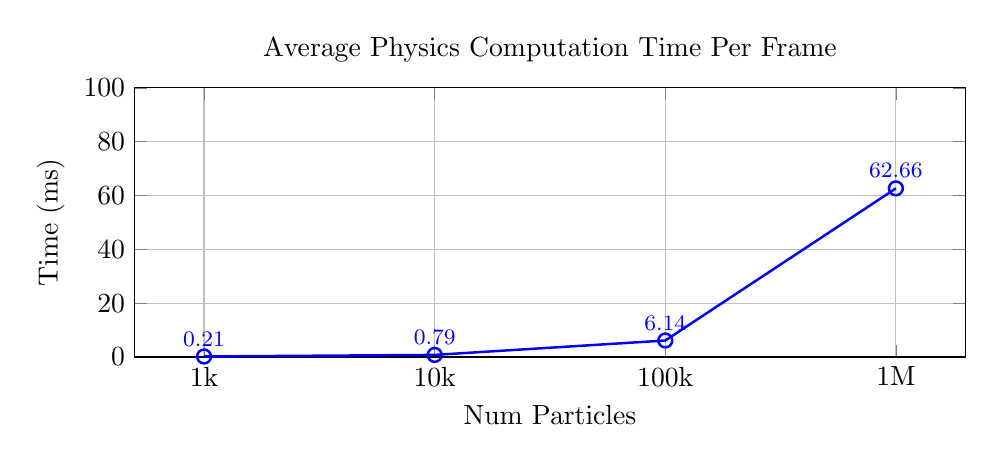
\begin{tikzpicture}
\begin{axis}[
  width=\linewidth, height=5cm,
  xlabel={Num Particles}, ylabel={Time (ms)},
  grid=both,
  symbolic x coords={1k,10k,100k,1M},
  xtick=data,
  ymin=0, ymax=100,
  nodes near coords,
  every node near coord/.append style={font=\footnotesize,anchor=south},
  title={Average Physics Computation Time Per Frame},
]
\addplot+[mark=o, line width=0.9pt, mark size=2.5pt]
  coordinates {(1k, 0.21) (10k, 0.79) (100k, 6.14) (1M, 62.66)};
\end{axis}
\end{tikzpicture}
\end{subfigure}

\vspace{0.7em}

\begin{subfigure}{\textwidth}
\centering
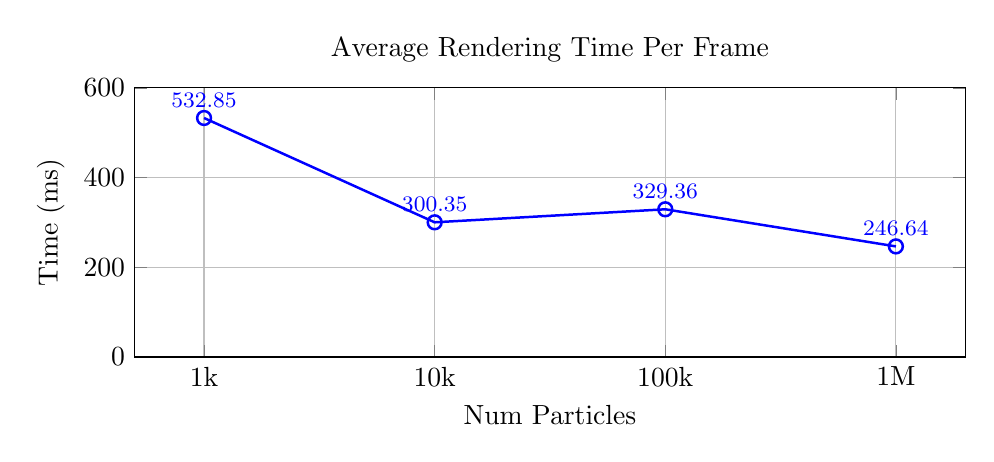
\begin{tikzpicture}
\begin{axis}[
  width=\linewidth, height=5cm,
  xlabel={Num Particles}, ylabel={Time (ms)},
  grid=both,
  symbolic x coords={1k,10k,100k,1M},
  xtick=data,
  ymin=0, ymax=600,
  nodes near coords,
  every node near coord/.append style={font=\footnotesize,anchor=south},
  title={Average Rendering Time Per Frame},
]
\addplot+[mark=o, line width=0.9pt, mark size=2.5pt]
  coordinates {(1k, 532.85) (10k, 300.35) (100k, 329.36) (1M, 246.64)};
\end{axis}
\end{tikzpicture}
\end{subfigure}
\hfill

\end{center}
\subsubsection{Spatial Grid Optimization}
\begin{center}

\begin{subfigure}{\textwidth}
\centering
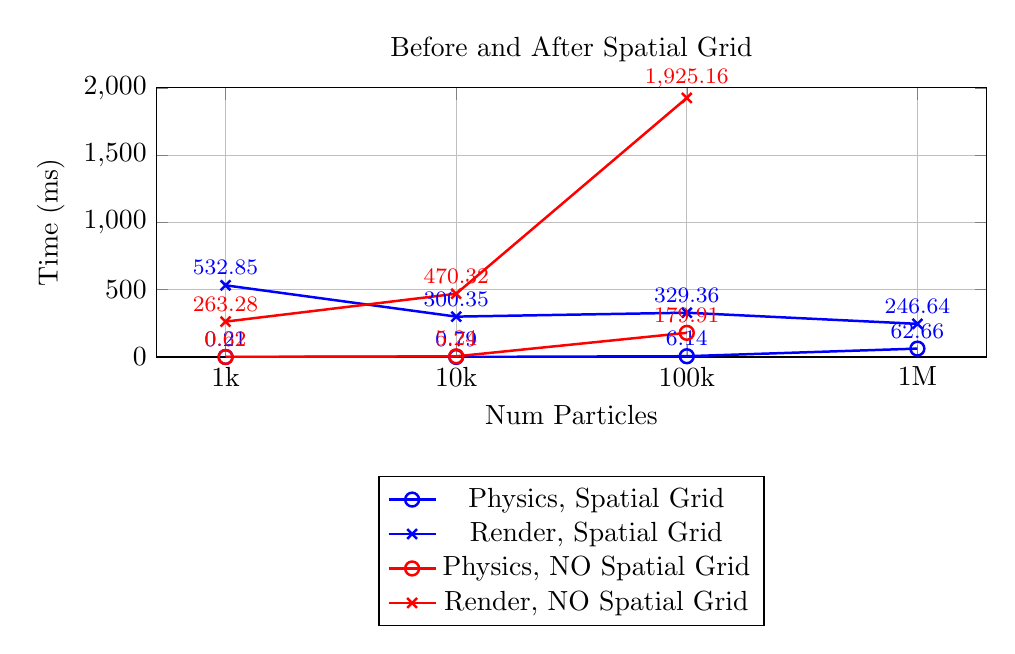
\begin{tikzpicture}
\begin{axis}[
  width=\linewidth, height=5cm,
  xlabel={Num Particles}, ylabel={Time (ms)},
  grid=both,
  symbolic x coords={1k,10k,100k,1M},
  xtick=data,
  ymin=0, ymax=2000,
  nodes near coords,
  every node near coord/.append style={font=\footnotesize,anchor=south},
  title={Before and After Spatial Grid},
  legend style={at={(.5,-1)}, anchor=south}  
]
\addplot+[color=blue, mark=o, line width=0.9pt, mark size=2.5pt]
  coordinates {(1k, 0.21) (10k, 0.79) (100k, 6.14) (1M, 62.66)};
\addlegendentry{Physics, Spatial Grid}  
\addplot+[color=blue, mark=x, line width=0.9pt, mark size=2.5pt]
  coordinates {(1k, 532.85) (10k, 300.35) (100k, 329.36) (1M, 246.64)};
\addlegendentry{Render, Spatial Grid}  

\addplot+[color=red, mark=o, line width=0.9pt, mark size=2.5pt]
  coordinates {(1k, 0.62) (10k, 5.24) (100k, 179.91)};
\addlegendentry{Physics, NO Spatial Grid}  
\addplot+[color=red, mark=x, line width=0.9pt, mark size=2.5pt]
  coordinates {(1k, 263.28) (10k, 470.32) (100k, 1925.16)};
\addlegendentry{Render, NO Spatial Grid} 

\end{axis}
\end{tikzpicture}
\end{subfigure}

\end{center}

\subsection{Discussion}

We include randomization in our initial locations for air particles, which may cause differences in number of collisions and computation costs.

\subsubsection{Problem Size}

First, we notice that the average physics computation time per frame increases as the number of particles increases. This is very expected. With the spatial grid optimization, the time for the physics step roughly follows the time complexity of $\mathcal{O}(N)$. From 10k particles onward, the physics computation time increases by roughly the same amount the as the number of particles. Before 10k particles, the problem size is very small and likely suffers from some of the overhead like transferring data to the GPU and initializing data. After 10k, it seems those costs get amortized away due to the large problem size.

Unlike the physics time, it seems that the rendering time generally went down as the problem size increased. Unlike the physics step, the rendering time was not dependent on the particle count. It had to render the same number of pixels regardless of the number of air particles. The render step also did not have much total variation, with a max of 532.85ms and a min of 246.64ms. We believe part of the changes are due to the random initial location for air particles. But the reason for the decreasing render time is likely because the time spent on physics is longer. Scheduling changes can allow the render step to overlap more with other work and partially "hide" some of the render step.

Overall, we can see that as problem size increases, computation time increases, but rendering time decreases.

Computation time increasing is expected, but earlier we found that calculating collision time should be approximately $O(N)$, meaning that scaling should look linear. However, we failed to take into account the closed space in which particles are compacted. The density of particles increases, which increases the number of neighbors we need to account for.

As for the GPU memory usage, it was very stable at around 210 MiB regardless of particle count. This is because the size of the image and world being calculated does not vary with particle count. It seems that the buffers allocated for that dominates the memory usage and the buffers allocated for the particles are relatively small in comparison.

\subsubsection{GPU}

Also, it is very interesting to note that our GPU utilization is very low (never exceeding 5\%). This suggests that either our problem size is too small, or we are not making effective use of the GPU, or our sampling script is not representative enough. Our problem involves many calculations that need to be done for 1 million particles, so we suspect that we likely are not making effective use of the GPU. In addition, while there are certainly improvements to be made, we believe that the GPU is reasonably engaged. 

Taking another look at our performance script, we realized that it samples for GPU utilization rather coarsely. More specifically, it only checks every 0.5 seconds. We believe that since we engage the GPU in bursts for the physics and render step, the performance script is often checking for GPU utilization when the GPU is not engaged. One takeaway from this is that we should make our performance script sample more often. But more importantly, we should likely even out our usage of the GPU. This could lead to a speedup by virtue of having a consistent and constant workload, instead of engaging the GPU in bursts.

\subsubsection{Limitations}

It is also worth noting synchronization in our program. When computing collisions with the ball, we must wait and synchronize between all threads for the net impulse on the ball. However, since all air particles are almost identical, the synchronization should not pose a large limitation to speedup.

In addition, we have an issue when too many particles are requested. Although the program should theoretically be capable of the calculations, once we reach around 3 million particles, the OpenGL window stops responding. We suspect this is a memory limitation of some sort. As a result, we capped ourself to 1 million particles.

\subsection{Deeper Analysis}

Using the spatial grid implementation with 1 million particles, the breakdown of our program time is as follows:

\begin{itemize}
\item Physics - 27.56\%
\item Render - 68.75\%
\item Overhead - 3.69\%
\end{itemize}

As you can see, our biggest bottleneck is in the render step. Unfortunately, there is a memory bandwidth issue here that we have to work around. In order to improve in this area, we need to optimize the data that we transfer between the CPU and the GPU. In exchange for decreasing accuracy, we can make time steps coarser. We can also attempt to only send particles that we know need to be updated to the GPU. In addition, we probably can also merge the physics and the render step. Currently, these are distinct kernel functions. That means that we must transfer data to the CPU after the physics step and then transfer data back to the GPU to start the render step. Instead, we may be able to merge these together to avoid two data transfers.

The physics step does not have too much room to improve without sacrificing accuracy. However, we did not get a chance to play around with grid parameters, which certainly could improve performance by reducing the number of particles to check. At this point, the physics step will mostly rely on parameter tuning for more gains.

We believe that our choice of machine for this project was pretty good. This project was computation heavy and some parts of it were embarrassingly parallel. However, the memory bandwidth between the device and host does pose a problem that will require some engineering. Compared to other setups though, such as single or multi-cpus, our setup will certainly outperform them. However, a setup with multiple GPUs would definitely be better than what we did.

\section{Work Distribution}

The division of work between Maxwell and Daniel is shown in Table 1. The work is roughly a 40\% (Maxwell) 60\% (Daniel) split.

\begin{table}[h!]
\centering
\begin{tabular}{ |c|c|c| }
 \hline
 Task & Maxwell & Daniel \\
 \hline
 Research/Develop Algorithm & X & X \\
 \hline
 Research Physics Formulas & X & X \\
 \hline
 Initialize Codebase &  & X \\
 \hline
 Setup Rendering & X &  \\
 \hline
 Sequential Implementation & X & \\
 \hline
 Parallel Implementation w/ CUDA & & X \\
 \hline
 Code Cleanup and Optimizations & & X \\
 \hline
 Proposal, Milestone, Final Report & X & X \\
 \hline
\end{tabular}
\caption{Division of project tasks.}
\label{tab:mytable}
\end{table}

\section{References}

Bird, G. A. Molecular Gas Dynamics and the Direct Simulation of Gas Flows. Oxford University Press, 1994.

Marion, Jerry B., and Stephen T. Thornton. Classical Dynamics of Particles and Systems. Brooks/Cole, 2012.

Halliday, David, Robert Resnick, and Jearl Walker. Fundamentals of Physics. Wiley, 2013.

Goldstein, Herbert, Charles Poole, and John Safko. Classical Mechanics. Addison-Wesley, 2002.



\end{document}
